\documentclass[a4paper]{report}
\usepackage{amsmath} 
\usepackage{graphicx}

\title{DDPG + HER in FetchPush-v1 Gym Environment with Python3 and Tensorflow 2.0}
\author{Simone De Angelis 1760464\\ Veronica Romano 1580844}
\date{\today}


\begin{document}

\maketitle

\chapter{Introduction and Work Purposes}
Reinforcement Learning is learning what to do and how to map situations to actions. The end result is to maximize the numerical reward. The learner is not told which action to take, but instead must discover which action will yield the maximum reward. As illustrated in Figure \ref{Fig: scheme}, an agent, which is who have to reach a goal, stars from a state $s_t$ and through actions $a_t$, manipulates the environment. From this it takes a reward $r_{t+1}$, if goes more close to the goal and it's intended to encourage good agent behavior, and discovers the next state $s_{t+1}$. These two are the reward and the state that permits the agent to re-implement the cycle. 

\begin{figure}[h!]
\centering
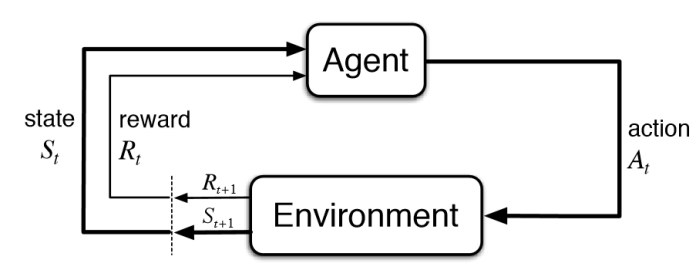
\includegraphics[scale=0.5]{reinforcement.jpg}
\caption{\label{Fig: scheme} Formulation of a basic Reinforcement Learning project.}
\end{figure}

This proceeds until the goal is reached. 

%Reinforcement Learning also differs from the other machine learning techniques. In fact in supervised learning there is a "supervisor" which has the knowledge of the environment and shares it with the agent to complete the task. while in reinforcement learning is the agent that learns from its own experience. Moreover there is a reward function which acts as a feedback to the agent. With respect to unsupervised learning where there is no mapping from input to output, in reinforcement learning the mapping is present. 
%This type of learning is usually modeled through Markov Decision Process. If the environment is non-deterministic we need a transition model $P(s'|s,a)$ and the utility function is the sum of the received rewards.

In few words, an \textit{agent} has a set of \textit{action space} which it can perform in a given \textit{environment} for which it gets \textit{rewarded} if that action meets some criteria. The agent learn to take actions for maximizing this reward.
This is the basic principle of reinforcement learning. In particular reinforcement learnin is a field of artificial intelligence that has several applications in the robotics field, which is the field of this project.

 
OpenAI Gym is a open source tool that allows us to work with algorithm for reinforcement. Previously there aren't many standard environment that could be used to the developed of these algorithms. In fact with the rise of Gym, reinforcement learning becomes more practical and implementable with respect to the traditional machine learning methods. Gym is available on the corresponding GitHub repository. On the other hand there is also MuJoCo (Multi-Joint dynamics with Contact). This is a physical engine for detailed, efficient rigid body simulations with contacts. It has a dynamic library with C/C++ API. mujoco-py allows using MuJoCo from Python3. It includes an XML parser, model compiler, simulator, and interactive OpenGL visualizer. To use it a specific license is needed; we use this for visualizing and using our environment, and to provide a graphical visualization of the results reached. MuJoCo is also customizable, so the environment can be modified by changing its XML code. This permits also to create new environments for implementing new tasks. However the best part is that MuJoCo provides the physical interactivity (like calculation of contact forces) which helps an engineer or researcher to test their model rigorously before moving to production.
\\


This work consists in implementing the FetchPush-v1 environment provided by Gym OpenAI (using MuJoCo as physical simulator), and by using a specific algorithm, which in our specific case is DDPG+HER, experimenting on this environment. Also a specific framework will be assigned for  implementing the code. All the result reached will be illustrated in Chapter \ref{exp}. While in the following sections we will exploit in details the algorithm used for our task, the environment, and the implementation framework.


\chapter{Implementation Assignment}
To implement this work a specific framework has been assigned. We have used Python3 and TensorFlow 2.0. In particular we used TensoFlow for building the neural networks for our actor and critic.

\section{DDPG + HER Algorithm}

\subsection{DDPG (Deep Deterministic Policy Gradient)}
Deep Deterministic Policy Gradient (DDPG) (illustrated in \cite{ddpg}) is a model-free, off-policy actor-critic algorithm using deep function approximators that can learn policies in high-dimensional, continuous action spaces. It concurrently learns a Q-function and a policy. As DPG, it uses off-policy data and the Bellman equation to learn the Q-function, and uses the Q-function to learn the policy. DDPG, being an actor-critic technique, consists of two models: Actor and Critic. The Actor is a policy network that takes the state as input and outputs the exact action (continuous), instead of a probability distribution over actions. So the actor function $\mu(s|\theta^{\mu})$ specifies the current policy by deterministically mapping states to a specific action. The Critic $Q(s,a)$ is a Q-value network that takes state and action as input and outputs the Q-value. It is learned using Bellman equation as in Q-learning. DDPG is used in the continuous action setting and the word "Deterministic" in DDPG refers to the fact that the actor computes the action directly instead of a probability distribution over actions. This approach is closely connected to Q-learning, and is motivated the same way: if you know the optimal action-value function $Q^*(s,a)$, then in any given state, the optimal action $a^*(s)$ can be found by solving:

\begin{equation}
a^*(s) = argmax_a Q^*(s, a)
\end{equation} 

DDPG put together the learning of an approximator $Q^*(s, a)$ and the learning of an approximator $a^*(s)$, and it does this in a way which is specifically for continuous action spaces. This refers to the way in which the $\max$ over actions is computed in $\max_a Q^*(s, a)$. When there are a finite number of discrete actions, the max poses no problem, because we can just compute the Q-values for each action separately and directly compare them. However, when the action space is continuous, we can't exhaustively evaluate the space, and solving the optimization problem is highly non-trivial. Because the action space is continuous, the function $Q^*(s,a)$ is presumed to be differentiable with respect to the action argument. This allows us to set up an efficient, gradient-based learning rule for a policy $\mu(s)$ which exploits that fact. Then, instead of running an expensive optimization subroutine each time we wish to compute $\max_a Q(s,a)$, we can approximate it with $\max_a Q(s,a) \approx Q(s,\mu(s))$.

As in DQN, DDPG uses a replay buffer which is a finite sized cache R. Transitions were sampled from the environment according to the exploration policy and the tuple $(s_{t}, a_{t}, r_{t}, s_{t+1})$ was stored in the replay buffer. When the replay buffer was full, the oldest samples were discarded. At each timestep the actor and critic are updated by sampling a minibatch uniformly from the buffer. The replay buffer can be large due to the fact that DDPG is an off-policy algorithm. It allows the algorithm to benefit from learning across a set of uncorrelated transitions. A copy of the actor and critic networks is created; respectively $Q'(s,a|\theta^{Q'})$ and $\mu'(s|\theta^{\mu'})$. These copies are used for calculating the target values. Also the weights of these target networks are updated slowly to make them following the learned networks. This means that the target values are constrained to change slowly, and this improves the stability of learning. The authors of \cite{ddpg} found that having both target $\mu'$ and $Q'$ is required to have stable targets in order to consistently train the critic without divergence. 
Moreover the main advantage of off-policy algorithms such as DDPG is that the exploration can be done independently from the learning algorithm. The exploration policy $\mu'$ is obtained by adding noise to our policy $\mu(s_{t}|\theta_{t}^{\mu})$.

\begin{figure}[h!]
\centering
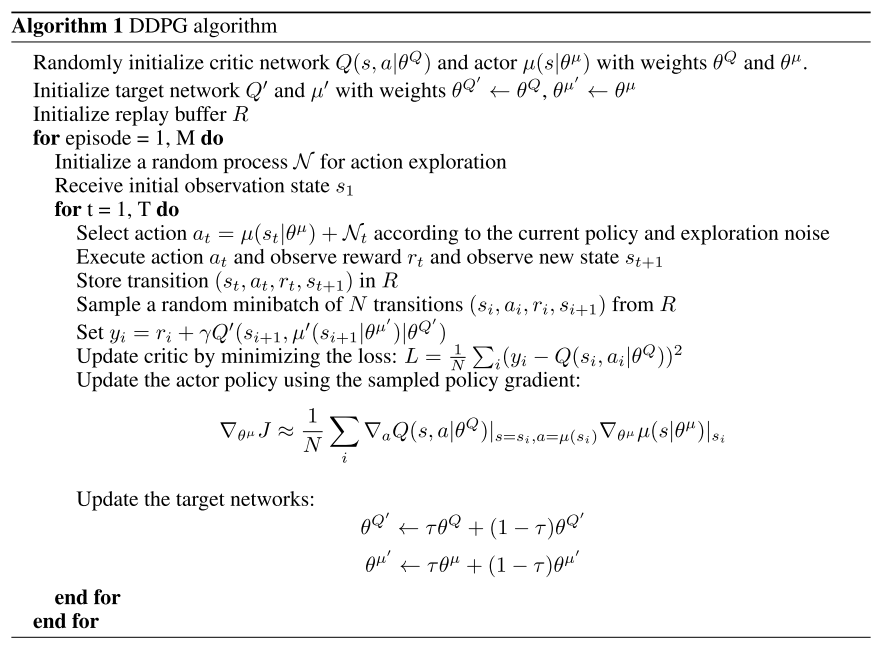
\includegraphics[scale=0.65]{ddpg.png}
\caption{\label{Fig: ddpg} Pseudocode of DDPG algorithm.}
\end{figure}

The Figure \ref{Fig: ddpg} shows the pseudocode of the algorithm.



\subsection{HER (Hindsight Experience Replay)}
Hindsight Experience Replay is a reinforcement learning algorithm which can learn from failure. It's been proven that HER can learn successful policies on most of the new robotics problems from only sparse rewards. In many tasks the first iteration is not a success or if it's so, it's probably only a lucky episode. A classical reinforcement algorithm will not learn anything from this experience since it just obtains a constant reward equal to -1, that does not contain any learning signal. HER allows to learn also from this type of experiences. In fact also if we have not succeeded at a specific goal, we have at least achieved a different one. We can imagine that we want to reach this new goal at the beginning instead of that we want to achieve originally. By doing this substitution, the reinforcement learning algorithm can obtain a learning signal since it has achieved some goal; even if it wasn't the one that we meant to achieve originally. If we repeat this process, we will eventually learn how to achieve arbitrary goals, including the goals that we really want to achieve. This technique is called Hindsight Experience Replay because it replays experience with goals which are chosen in hindsight, after the episode has finished. More deeply, the idea behind HER is that after experiencing some episode we store in the replay buffer every transition from a state to the following, not only with the original goal used for this episode but also with a subset of other goals. The goal will influence only the agent's action and therefore we can replay each trajectory with an arbitrary goal assuming that we use an off-policy algorithm like DDPG. One important aspects is the choice of the additional goals used for replay. In the simplest version the goal is substituted with the goal achieved in the final state of the episode. Another version is to choose the goal in a random way. The complete algorithm of HER is illustrated in Figure \ref{Fig: her}

\begin{figure}[h!]
\centering
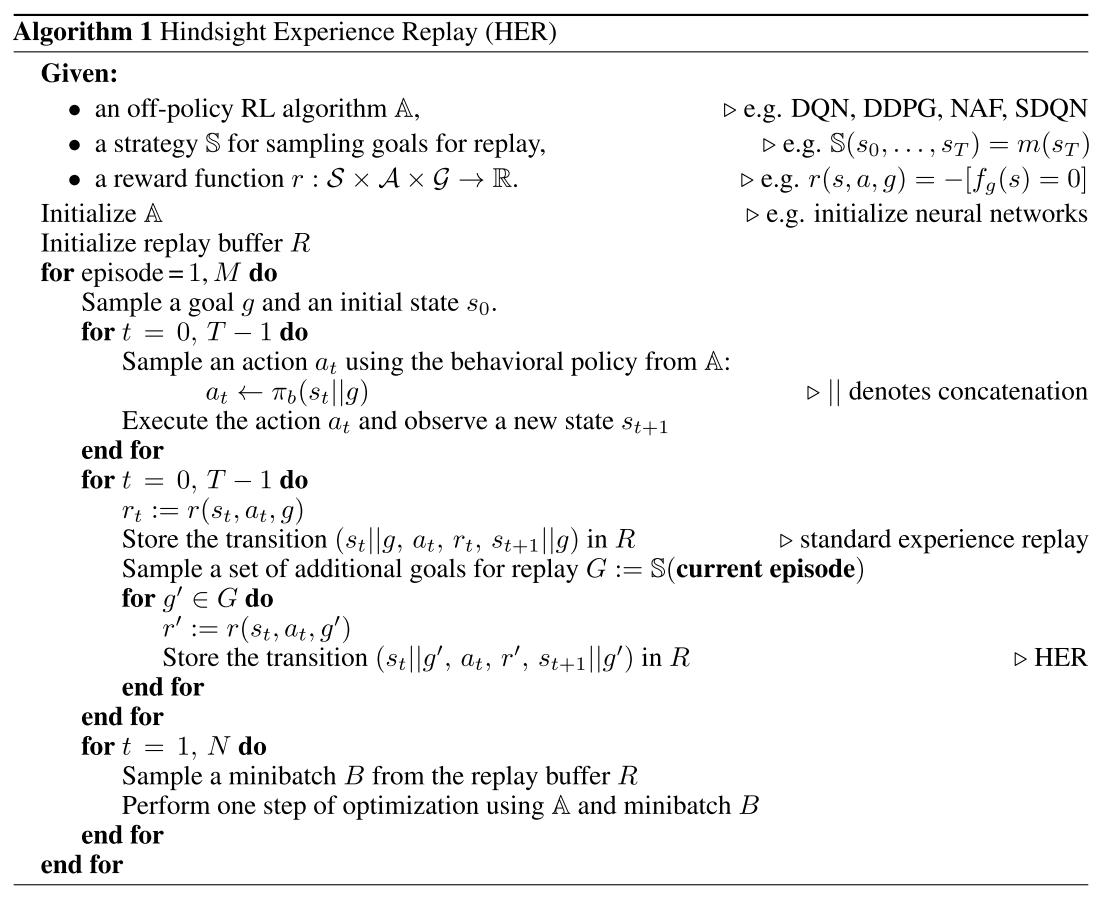
\includegraphics[scale=0.5]{her.png}
\caption{\label{Fig: her} Pseudocode of HER algorithm.}
\end{figure}

In \cite{her} to show the performances of HER, are used different Fetch environments including FetchPush. In this paper, the DDPG algorithm is used for performing training with Adam as optimizer, as in our case. Also in this paper is shown that DDPG without HER is unable to solve any of the tasks. It confirms that HER is a crucial element which makes learning from sparse, binary rewards possible. Moreover it also states that DDPG+HER performs better even if the goal state is identical in all episodes. In \cite{her} are also shown several strategies for choosing goals to use with HER. As mentioned one strategy is to choose the goal corresponding to the final state of the environment (\textit{final} strategy). Other strategies are:
\begin{itemize}
\item \textit{future} that replays with k random states which come from the same episode as the transition being replayed and were observed after it
\item \textit{episode} that replays with k random states coming from the same episode as the transition being replayed
\item \textit{random} that replays with k random states encountered so far in the whole training procedure
\end{itemize}

All of these strategies have a hyperparameter k which controls the ratio of HER data to data coming from normal experience replay in the replay buffer. In the paper is shown that all these strategies excluded the \textit{random} one are able to solve pushing task regardless the value of k.

\subsection{DDPG and HER work together}
HER works very well in goal-based environments with sparse rewards. Vanilla DDPG and DDPG+HER have been compared.  This comparison includes the sparse and the dense reward versions of the environment. Has been shows that DDPG+HER with sparse rewards outperforms significantly Vanilla DDPG with sparse or dense rewards and DDPG+HER with dense rewards. There results are exposed in \cite{multigoal}. This paper in fact evaluates the performance of DDPG with and without HER on all the Fetch and HandManipulateBlock environments. 

\begin{figure}[h!]
\centering
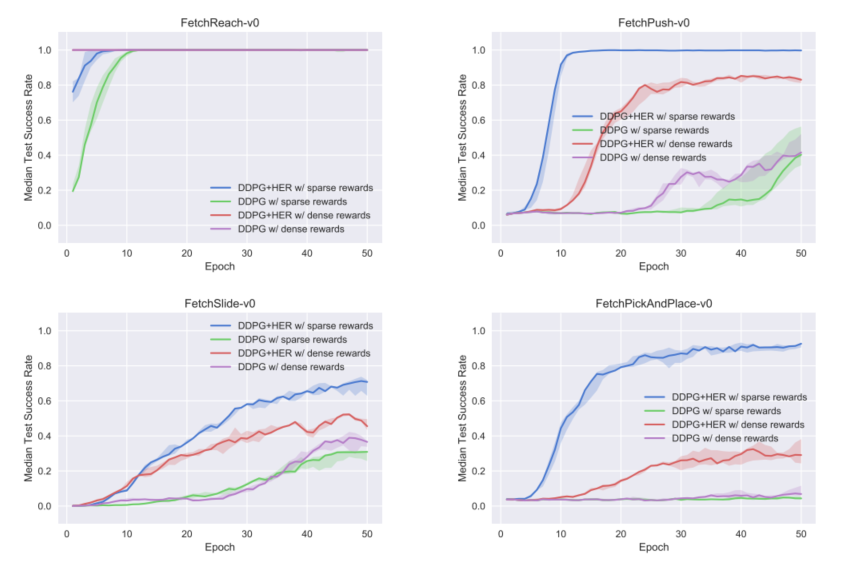
\includegraphics[scale=0.65]{fetchcomparison.png}
\caption{\label{Fig: comparison} This Figure illustrates the comparison between Vanilla DDPG and DDPG+HER with sparse and dense rewards in all four Fetch environments provided by OpenAI Gym.}
\end{figure}

The results reached for Fetch environments, in which we are mainly interested, are illustrated in Figure \ref{Fig: comparison}. It depicts the median test success rate for all four Fetch environments. FetchReach-v0 is clearly a very simple environment and can easily be solved by all four configurations. On the remaining environments, DDPG+HER clearly outperforms all other configurations. Interestingly, DDPG+HER performs best if the reward structure is sparse but is also able to successfully learn from dense rewards. For vanilla DDPG, it is typically easier to learn from dense rewards with sparse rewards being more challenging. Moreover, as we can see from the Figure \ref{Fig: comparison}, for FetchPush-v0 environment the combined approach DDPG+HER with sparse reward is that reached better performance and better success rate. the authors believe that a possible reason why DDPG+HER typically performs better with sparse rewards is mainly due to the following two reasons. The first reason is that learning the critic is much simpler for sparse rewards. In the dense case, the critic has to approximate a highly non-linear function that includes the euclidean distance between positions and the difference between two quaternions for rotations. On the other hand, learning the sparse return is much simpler because the critic has only to differentiate between success and failed states.
The second reason is that a dense reward biases the policy to a specific strategy. The dense reward however encourages the policy to chose a strategy that achieves the desired goal directly
 


\section{Gym Environment}
The release provided by OpenAI Gym, contains four environments using the Fetch research platform. These environments use the MuJoCo physics simulator. Our environment is, as previously mentioned, FetchPush-v1 (Figure \ref{Fig: fetchpush}). Fetch goal is to move a box by pushing it until it reaches a desired goal position. This tasks has the concept of a "goal". By default it uses a sparse reward of -1 if the desired goal was not yet achieved and 0 if it was achieved (within some tolerance). This because the sparse rewards are more realistic in robotics applications and the developers encourage their use.

\begin{figure}[h!]
\centering
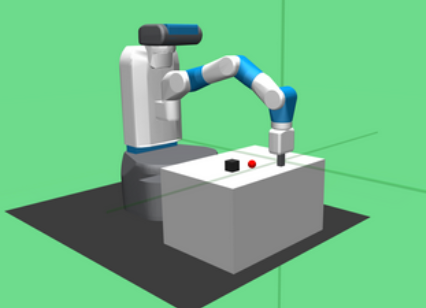
\includegraphics[scale=0.5]{fetchpush.png}
\caption{\label{Fig: fetchpush} FetchPush-v1 Gym environment.}
\end{figure}

The Fetch environment is based on the 7-DoF Fetch robotics arm which has a two-fingered parallel gripper that are locked to prevent grasping. The learned behavior
is usually a mixture of pushing and rolling. The goal is 3-dimensional and describes the desired position of the object (or the end-effector for reaching). Rewards are sparse and binary in fact the agent obtains a reward of 0 if the object is at the target location and −1 otherwise. Actions are 4-dimensional: 3 dimensions specify the desired gripper movement in Cartesian coordinates and the last dimension controls opening and closing of the gripper that in FetchPush-v1 is always closed. However in other environments, like FetchPickandPlace-v1, this last dimension is very relevant for the task.
Observations include the Cartesian position of the gripper, its linear velocity as well as the position and linear velocity of the robot's gripper. If an object is present, we will have also the object's Cartesian position and rotation using Euler angles, its linear and angular velocities, but also the position and linear velocities relative to gripper.
The observation space is of type gym.spaces.Dict space, with at least three keys that are:
\begin{itemize}
\item observation: The actual observation of the environment, for example robot state and position of objects.
\item desired\_goal: The goal that the agent has to achieve. In FetchPush-v0 would be the 3-dimensional target position on which we would like the box will be
\item achieved\_goal: The goal that the agent has currently achieved instead. Ideally, this would be the same as desired\_goal as quickly as possible.
\end{itemize}




\chapter{Experiments and Results \label{exp}}

As previously  mentioned, our work consisted of exploring in FetchPush-v1 environment, implementing the algorithm DDPG+HER. To implement our work we write a code in Python3 and TensorFlow 2.0. The code is structured in this way:

\begin{itemize}
\item a \textit{buffer.py} file in which is implemented the replay buffer in which the transition are stored. These transitions include state, action, reward, actual state, a flag \textit{done} and the goal. This transition will be then used to define the new goals for HER implementation.

\item a \textit{networks.py} file in which the actor and critic networks are created by following the conventional parameters used in this case of tasks found on several papers regarding this argument. The networks are created by using \textit{tensorflow.keras} and are formed by only dense layers with \textit{relu} as activation function, and a final critic dense output layer without activation function, and a final actor dense output layer with \textit{tanh} as activation function.

\item a \textit{ddpg\_tf2.py} file in which all the parameters for the agent are defined and the DDPG algorithm is implemented. Here are also initialized the target actor and target critic networks. The \textit{adam} optimizer is also defined with different learning rate for actor and critic networks.

\item a \textit{main\_ddpg.py} file in which we have defined our environment. To the agent are provided the environment, the dimension of the \textit{observation} space as input dimension, the dimension of the \textit{desired\_goal} and the \textit{action\_space} dimension. 

\end{itemize}

\begin{thebibliography}{}

\bibitem{multigoal}
Plappert, Matthias, et al. "Multi-goal reinforcement learning: Challenging robotics environments and request for research." arXiv preprint arXiv:1802.09464 (2018).

\bibitem{her}
Andrychowicz, Marcin, et al. "Hindsight experience replay." Advances in neural information processing systems. 2017.

\bibitem{ddpg}
Lillicrap, Timothy P., et al. "Continuous control with deep reinforcement learning." arXiv preprint arXiv:1509.02971 (2015).

\end{thebibliography}


\end{document}